\documentclass[a4paper, 12pt,oneside]{article} 
%\documentclass[a4paper, 12pt,oneside,draft]{article} 
\usepackage{preamble_bis}
%--------------------- ACTUAL FILE ---------------------- %
\begin{document} 
%%%
	\begin{titlepage}
    \newcommand{\HRule}{\rule{\linewidth}{0.5mm}} % Defines a new command for the horizontal lines, change thickness here
    
    \center  % Center everything on the page
     
    %----------------------------------------------------------------------------------------
    %   HEADING SECTIONS
    %----------------------------------------------------------------------------------------
    
    \vspace{3cm}
    \textsc{\LARGE École polytechnique fédérale de Lausanne}\\[1.5cm] % Name of your university/college
    
    \textsc{\Large Project N$^\circ$2 Report}\\[0.5cm] % Major heading such as course name
    \textsc{\large Randomized Nystr\"om
    }\\[0.5cm] % Minor heading such as course title
    
    %----------------------------------------------------------------------------------------
    %   TITLE SECTION
    %----------------------------------------------------------------------------------------
    
    \HRule \\[0.4cm] % line above and under the title
    
    
    % Title of your document
    
    \HRule \\[1.5cm]
     
    %----------------------------------------------------------------------------------------
    %   AUTHOR SECTION
    %----------------------------------------------------------------------------------------
    
    \begin{minipage}{0.4\textwidth}
    \begin{flushleft} \large
    
    \emph{Authors:}\\
    Tara \textsc{Fjellman}\\
    Amal \textsc{Seddas}\\
    
    
    
    
    \end{flushleft}
    \end{minipage}
    ~
    \begin{minipage}{0.4\textwidth}
    \begin{flushright} \large
    
    \emph{Professor:} \\
    Laura \textsc{Grigori
     }\\
    \end{flushright}
    \end{minipage}\\[10cm]
    %
    
    
    %----------------------------------------------------------------------------------------
    %   LOGO SECTION
    %----------------------------------------------------------------------------------------
    
    
\includegraphics[width=0.4\linewidth]{Logo-1 .pdf}\\[1cm] 
    % Include a department/university logo - this will require the graphicx package
     
    %----------------------------------------------------------------------------------------
    
    \vfill % Fill the rest of the page with whitespace
    
    \end{titlepage} 
	% Add titlepage
	\clearpage
	\tableofcontents
	\thispagestyle{empty}
	% Add table of contents
	\clearpage
	\pagenumbering{arabic}
	\setcounter{page}{1}

	\section{Introduction}
		\lipsum[1]
	\section{Randomized Nyström low rank approximation}
		The goal of the Randomized Nystr\"om Algorithm is to represent a given matrix $A \in \mathbb{R}^{n \times n}$ by some approximated matrix with a lower rank $k < n$. The starting point of the algorithm is a rank-$\ell$ approximation of $A$, in the form
\[
A_{Nyst} := (A\Omega)(\Omega^T A \Omega)^{\dagger}(\Omega^T A) \in \mathbb{R}^{n \times n},
\]
where $(\Omega^T A \Omega)^\dagger$ is the pseudoinverse of $\Omega^T A \Omega$ and $\Omega \in \mathbb{R}^{n \times \ell}$ is a sketching matrix. We assume $k < \ell < n$. To further reduce the rank of $A_{Nyst}$ to $k$, we have two choices: approximate only the core matrix $\Omega^T A \Omega$ or the whole $A_{Nyst}$. In this project, we focus on the second approach. Algorithm \ref{alg:nystrom} shows how this can be achieved.

\begin{algorithm}
\caption{Randomized Nystr\"om approximation using the Cholesky decomposition}
\label{alg:nystrom}
\begin{algorithmic}[1]
  \State Let $C = A\Omega$ and $B = \Omega^T C$.
  \State Compute the Cholesky decomposition: $B = LL^T$.
  \State Solve the linear system using back substitution: $Z = C(L^T)^{-1}$.
  \State Perform QR decomposition: $Z = QR$.
  \State Compute the singular value decomposition (SVD) of $R$ and truncate:
  \[ R = U \Sigma V^T \approx \tilde{U}_k \tilde{\Sigma}_k \tilde{V}_k^T. \]
  \State Set $\tilde{U}_k = Q\tilde{U}_k$ (or equivalently $\tilde{U}_k = Z\tilde{V}_k\tilde{\Sigma}_k^{-1}$) and return $\tilde{U}_k \tilde{\Sigma}_k^2 \tilde{U}_k^T \approx A_{Nyst}$.
\end{algorithmic}
\end{algorithm}

To show why the result of Algorithm \ref{alg:nystrom} is in fact a rank-$k$ approximation of $A_{Nyst}$, we write
\begin{align*}
\tilde{U}_k \tilde{\Sigma}_k^2 \tilde{U}_k^T &= Q\tilde{U}_k \tilde{\Sigma}_k \tilde{\Sigma}_k^T \tilde{U}_k^T Q^T \\
&\approx QRR^T Q^T = ZZ^T = A\Omega(L^T)^{-1}(L^T)^{-1}\Omega^T A^T \\
&= A\Omega(LL^T)^{-1}\Omega^T A^T = A(\Omega^T A \Omega)^{\dagger}\Omega^T A^T.
\end{align*}

However, here we have the inverse of $\Omega^T A \Omega$ instead of its pseudoinverse. Unfortunately, Algorithm \ref{alg:nystrom} fails in Step 2 if $\Omega^T A \Omega$ is numerically singular. In this case, as in \cite{reference}, we replace $L$ by a square root of $B$ in SVD form. Specifically, we write $B = U_B \Sigma_B U_B^T$ (since $B$ is SPSD), and set $L = U_B \sqrt{\Sigma_B} U_B^T$. By construction, we have
\[
LL^T = U_B \sqrt{\Sigma_B} U_B^T (U_B \sqrt{\Sigma_B} U_B^T)^T = U_B \Sigma_B U_B^T = B.
\]
We then replace $(L^T)^{-1}$ with $(L^T)^\dagger$. This can be simply calculated as
\[
(L^T)^\dagger = (U_B \sqrt{\Sigma_B} U_B^T)^\dagger,
\]
where $\sqrt{\Sigma_B}$ is a diagonal matrix whose entries are given by
\[
(\sqrt{\Sigma_B})_{i,i} = \begin{cases} \frac{1}{(\sqrt{\Sigma_B})_{i,i}} & \text{if } (\sqrt{\Sigma_B})_{i,i} \neq 0, \\
0 & \text{otherwise.} \end{cases}
\]
\section{Sketching and Sketching Matrices}

In this section, we provide a detailed overview of sketching and the sketching matrices utilized in this project. The concept of sketching involves transforming a high-dimensional matrix $A \in \mathbb{R}^{n \times n}$ into a lower-dimensional representation $A\Omega$, where $\Omega \in \mathbb{R}^{n \times \ell}$ is a tall and skinny sketching matrix. The goal of sketching is to embed the high-dimensional data into a reduced-dimensional space while preserving the essential geometric properties of the data.

More formally, given any two vectors $x$ and $y$ in the high-dimensional space, their sketched counterparts $\hat{x}$ and $\hat{y}$ should approximately preserve their inner product:
\begin{equation}\label{eq:1}
\left| \langle \hat{x}, \hat{y} \rangle - \langle x, y \rangle \right| \leq \varepsilon \|x\|_2 \|y\|_2 \tag{2}
\end{equation}
where $\varepsilon > 0$ is a small approximation error. However, achieving this exact preservation for all $x$ and $y$ is generally infeasible due to the reduced dimensionality $\ell$. Instead, $\Omega$ is typically chosen randomly, ensuring that \cref{eq:1} holds with high probability $1 - \delta$, where $\delta < 1$.

In this project, we employ two specific types of sketching matrices:
\subsection{Gaussian sketching }
The Gaussian sketching matrix is a widely used random projection method in which the entries of the sketching matrix $\Omega$ are drawn independently from a standard normal distribution. Mathematically, it is defined as:
\[
\Omega_{ij} \sim \mathcal{N}(0, 1),
\]
where $\Omega \in \mathbb{R}^{n \times \ell}$, and $\ell$ represents the reduced dimensionality of the sketch.

The sketched matrix $A\Omega$, for an input matrix $A \in \mathbb{R}^{n \times d}$, satisfies approximate preservation of the geometry of the original matrix. Specifically, the sketch guarantees that for any vector $x \in \mathbb{R}^d$:
\[
(1 - \varepsilon)\|A x\|_2^2 \leq \|A \Omega x\|_2^2 \leq (1 + \varepsilon)\|A x\|_2^2,
\]
with high probability, where $\varepsilon > 0$ is a small approximation error. This property ensures that pairwise distances between points in the projected space are approximately preserved.

The Gaussian sketching matrix can also be viewed as a random transformation that approximately satisfies the following subspace embedding property for any subspace $T \subseteq \mathbb{R}^d$:
\[
(1 - \varepsilon) \|v\|_2^2 \leq \|\Omega v\|_2^2 \leq (1 + \varepsilon) \|v\|_2^2, \quad \forall v \in T.
\]

\section{Block Subsampled Randomized Hadamard Transform (BSRHT)}

\subsection{Subsampled Randomized Hadamard Transform (SRHT)}
The BSRHT is a version of the Subsampled Randomized Hadamard Transform (SRHT) specifically designed for distributed architectures. For $n$ being a power of two, the SRHT can be defined as
\[
\Omega^T = \sqrt{\frac{n}{\ell}} RHD,
\]
where:
\begin{itemize}
  \item $H \in \mathbb{R}^{n \times n}$ is the normalized Walsh--Hadamard matrix, which is defined recursively as:
  \[
  H_2 = \begin{pmatrix} 1 & 1 \\
  1 & -1 \end{pmatrix}, \quad H_n = \begin{pmatrix} H_{n/2} & H_{n/2} \\
  H_{n/2} & -H_{n/2} \end{pmatrix}, \quad \text{and} \quad H = n^{-1/2} H_n.
  \]
  \item $D \in \mathbb{R}^{n \times n}$ is a diagonal matrix with i.i.d. random variables $\sim \text{Uniform}(\pm 1)$.
  \item $R \in \mathbb{R}^{\ell \times n}$ is a subset of $\ell$ randomly sampled rows from the $n \times n$ identity matrix.
\end{itemize}

Note that we can always zero-pad the data to ensure that $n$ is a power of two. Now, for $P$ different processors, the BSRHT can be constructed block-wise from the SRHT as:
\[
\Omega^T = \begin{pmatrix} \Omega_1^T \\
\Omega_2^T \\
\vdots \\
\Omega_P^T \end{pmatrix} = \sqrt{\frac{n}{P\ell}} \begin{pmatrix} D_{L1} & \cdots & D_{LP} \end{pmatrix}
\begin{pmatrix}
RH & \cdots & 0 \\
\vdots & \ddots & \vdots \\
0 & \cdots & RH
\end{pmatrix}
\begin{pmatrix} D_{R1} & \cdots & 0 \\
\vdots & \ddots & \vdots \\
0 & \cdots & D_{RP} \end{pmatrix}, \tag{2}
\]
with:
\begin{itemize}
  \item $H \in \mathbb{R}^{n/P \times \ell/P}$ being the normalized Walsh--Hadamard matrix.
  \item $D_{Li} \in \mathbb{R}^{n/P \times n/P}$, $D_{Ri} \in \mathbb{R}^{n/P \times n/P}$ being diagonal matrices with i.i.d. Rademacher entries $\pm 1$.
  \item $R \in \mathbb{R}^{\ell \times n/P}$ being a uniform sampling matrix, sampling along the rows.
\end{itemize}

This structure is particularly suited for distributed computations, as it allows for parallelism while maintaining the theoretical properties of the SRHT.


	\section{Stability analysis}
		- bullet points about comments to include 
	\section{Parallelisation}
	We parallelise the algorithm by distributing among the processors the computation of $A \Omega,\Omega^T A \Omega$, and all other matrix operations with complexities at least proportional to $n$. 
	
	The parallelisation of QR factorisation was the topic of the first project. We therefore included the relevant functions for it in the code folder. The parallelisation of matrix products was however implemented from scratch. It was done as 	
	
	$$
	S=\left(\begin{array}{lll}
	S_{0} & S_{01} & S_{02} \\
	S_{10} & S_{11} & S_{12} \\
	S_{20} & S_{21} & S_{22}
	\end{array}\right), \quad \Omega=\left(\begin{array}{l}
	T_0 \\
	T_1 \\
	T_2
	\end{array}\right),
	$$
	with processor $i$ having the $i$-th row of $S$ and the $i$-th block row of $T$. Then

	\begin{algorithm}
		\caption{Computes the matrix product of two matrices $D$ and $E$ in parallel.}
		\begin{algorithmic}
		\Require $q$ is an integer and the square root of the number of processors, $D$ is an $m\times m$ matrix distributed such that processor $i$ has $D_{i//q,i\text{ mod }q}$ and $E$ is a $m\times n$ matrix distributed such that processor $i$ has $E_{i//q}$. FullProd is true if we also want to compute $E^TDE$.
		\Ensure $F=DE$ (and $G=E^TF$ too if FullProd is true). 
		\State $F_{ij} \gets P_{ij}E_j$
		\If{\text{FullProd}}
			\State $G_{ij} \gets E_i^FP_{ij}$
		\EndIf		
		\State Row-wise Sum-reduce : $F_i\gets \sum_j^q F_{ij}$
		\State Column-wise Gather on rank 0 : $F\gets [F_1^T,...,F_q^T]^T$
		\If{\text{FullProd}}
			\State Sum-reduce : $G\gets \sum_{i,j}^{q,q} G_{ij}$
		\EndIf
		%\Comment{Locally on rank 0}
		\end{algorithmic}
	\end{algorithm}
	$A \Omega,\Omega^T A \Omega$ multiplications were implemented 
	The matrix $A$ is distributed among processors by using a two-dimensional block distribution while the matrix $\Omega$ is distributed using a block row distribution. The parallelization of the algorithm is implemented in the following way:
	Describe how you parallelize randomized Nyström and provide pseudo-code of the parallel algorithm. For the parallelization, the matrix $A$ should be distributed among processors by using a two-dimensional block distribution while the matrix $\Omega$ should be distributed using a block row distribution. You can consider that the number of processors is a power of 2 such that you can easily distribute the matrices among processors. For example, when $P=\sqrt{P} \times \sqrt{P}=9$, the matrices $A$ and $\Omega$ are distributed as:



	$$
	B=\Omega^T A \Omega=\left(\begin{array}{lll}
		\Omega_1^T & \Omega_2^T & \Omega_3^T
		\end{array}\right)\left(\begin{array}{lll}
		A_{11} & A_{12} & A_{13} \\
		A_{21} & A_{22} & A_{23} \\
		A_{31} & A_{32} & A_{33}
		\end{array}\right)\left(\begin{array}{l}
		\Omega_1 \\
		\Omega_2 \\
		\Omega_3
		\end{array}\right)
	$$

	\begin{algorithm}
		\caption{Randomized Nystr\"om algorithm. The syntax was adapted from this Overleaf example.}\label{alg:parallel-rand-nystrom}
		\begin{algorithmic}
		\Require $A$ is an $n\times n$ symmetric positive semidefinite matrix, $\Omega$ is a sketching matrix of size $n\times l$, and $k$ is the rank of the approximation
		\Ensure $[A_{N y s t}]_k$, the rank-$k$ randomized Nystr\"om approximation of $A$. 
		\State $C \gets A \Omega$
		\State $B \gets \Omega^T C$
		\State $L, \text{Failed} \gets \text{Cholesky}(B)$ \Comment{Locally on rank 0}
		\If{Failed}
			\State $U, \Lambda \gets \text{EigDecomp}(B)$ \Comment{Locally on rank 0}
			\State $B_k^{+} \gets U(:,1:k) \Lambda(1: k, 1: k)^{+} U(:, 1: k)^T$
			\State $Q, R \gets \text{QR}(C)$ \Comment{Using TSQR}
			\State $\hat{U}_k \gets Q U(:, 1:k)$ \Comment{In parallel}
			\State $[A_{N y s t}]_k \gets \hat{U}_k \Lambda(1: k, 1: k)^{+} \hat{U}_k^T$ \Comment{In parallel}
		\Else{}
			\State $Z \gets C L^{-T}$ \Comment{Computed by substitution : $(LZ^T)^T=C^T$}
			\State $Q, R \gets \text{QR}(Z)$ \Comment{Using TSQR}
			\State $U_k, \Sigma_k, V_k \gets \text{TruncSVD}(R)$
			\State $\hat{U}_k \gets Q U(:, 1:k)$ \Comment{In parallel}
			\State $[A_{N y s t}]_k \gets \hat{U}_k \Sigma^2(1: k, 1: k) \hat{U}_k^T$ \Comment{In parallel}
		\EndIf
		\end{algorithmic}
	\end{algorithm}
	
	\section{Experimental procedure}
		- averaging to increase precision of results
		- when running in parallel, was simited by number of cores $p=2^{2s}$ with $s\in\mathbb{N}$ (due to perfect square constraint of the paralelised matrix multiplication and the SHRT algorithm using the Hadamard transform), so we ran results for 1,4,16,64
		- ran results on the Helvetios cluster 
		- $k$ was taken often around $n/20$ as we deemed this value relevant for real applications
		- n was made vary as powers of $2$ due to the Hadamard transformation while $l$ was taken logaritmically spaced just to make the visuals more easy to interpret  
	\section{Algorithm Performance}
        \subsection{Sequential Performance}
		- in general (both plots) observe that k rank approximation represents minority of runtime (as expected as of order $k^3 +nk^2$). Indeed for shown examples represents at most 10\%. This would be different if one were to take big values of $k$. Also does not really seem to depend on sketching method which makes sense given the computations are the same regardless of which sketching method was used to obtain the B and C matrices
		\begin{figure}[htb]       
			\centering             
				\vspace{0em}
				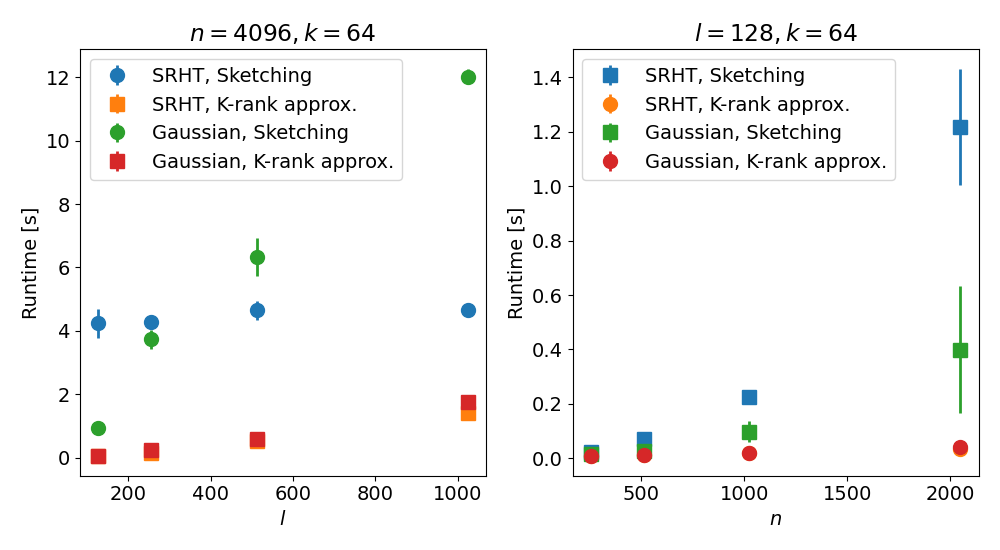
\includegraphics[width=.975\textwidth]{runtimes_l_n_variation}
				\caption{Runtimes associated to the tested sketching methods : as a function of $l$ (left) and as a function of $n$ (right). Runtimes are broken down in that associated to the computation of $A\Omega,\Omega^T A\Omega$ and that associated to the computation of the $k$ rank approximation.}
				\label{fig:runtimes-l-n-variation}
		\end{figure}

		- different behaviours as a function of l and n : as a function of l SRHT looks almost flat, having really slow increase, while gaussian increases steadily given its complexity is or order $nl^2 + ln^2$. This gives advantage for SRHT if we are embedding "dense spaces" as it scales much better than gaussian as function of l. For n : both algos show significant increase, but SRHT shows faster runtime growth. This makes sense due to extra $\log_2(n)$ term in its complexity. This would give advantage to gaussian sketching if we are dealing with sparse information within really high dimensional spaces.
		- 
        \subsection{Parallel Performance}
		- selected $l=n/64$ given we are using TSQR for the QR factorisation and we need the matrix to be tall-skinny to actually observe a speed-up. To have a good speed-up for a bigger $l$, while keeping numerical stability for ill-conditionned matrices another algo should be used.

		- for small example : some speed-up is observed as a function of number of cores but communication costs are non neglectable and even dominate the total runtime for p=64. This is expected as the computation is rather small to be run in parallel. The runtimes for the k-rank are the most affected as these represented the smallest part of the computation to start with. for the specific values selected the gaussian sketching is faster (indeed $l$ is taken only as a small fraction of $n$).

		\begin{figure}[htb]       
			\centering             
				\vspace{0em}
				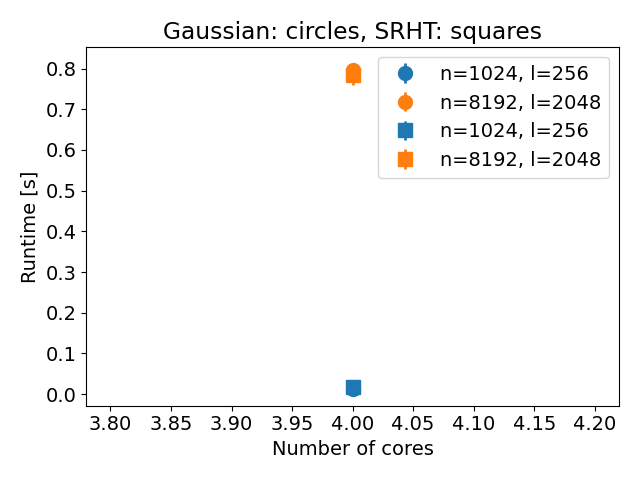
\includegraphics[width=.975\textwidth]{runtimes_cores_variation}
				\caption{Runtimes associated to the tested sketching methods as a function of the number of cores : for a ``small'' example (left) and a ``large'' one (right). Runtimes are broken down in that associated to the computation of $A\Omega,\Omega^T A\Omega$ and that associated to the computation of the $k$ rank approximation.}
				\label{fig:runtimes-cores-variation}
		\end{figure}
		- for the large : communication is not much of an issue, and big speed ups (quasi linear) are observed for the sketching computation. This means the parallelization is successful and scales well for big computations. We can see the speedup is not as good for k-rank partly because the computation was smaller to start with. The fact that the matrix is not that tall-skinny is also expected to have contributed to the low speed-up of that part.
		- 

	\section{Conclusion}
	\section*{Aknowledegments}
	\section*{References}
	%\appendix
	%	\section{Runtime Estimation}\label{appendix:runtime_estimation}
%%%
\end{document} 